\graphicspath{{../images/ch6/}}	% Image directory


\chapter{Hybrid resistive-pulse optical detections in microfluidic systems}
\label{chap:rpim}

	

	\section{Background \& Theory}
		
		As we have seen, RP sensing is a method for determing the physical properties of particles by way of measuring the change in resistance of a conducting channel they create as they pass through it. RP's primary advantage is that it can be employed at many scales and in a diverse number of applications, and is especially useful at the nanoscale where the number of particle characterization techniques is limited---in particular, optical imaging is prohibited at this scale. To first order, the mechanism for the rp current pulses is straight forward: when the particle enters the channel, it occupies a volume that would otherwise be occupied by ions, decreasing the conductance, and increasing the total system resistance. According to this simple model, the resistive of the system is determined solely by the equation
		
		\begin{equation}\label{eq:resistance}
			R=\rho\int A^{-1}\left(x\right) dx,
		\end{equation}
		
		where $R$ is the system resistance, $A\left(x\right)$ is the annular cross-section of the channel at position $x$, and $\rho$ is the resistivity of the solution. In most RP set ups, the current is measured instead of the resistance, so Eq. \ref{eq:resistance} is usually inverted via Ohm's law to obtain the current: $\Delta I/I_{p}=\Delta R/R_{0}$, where $I$ is the measured current, and the subscripts $0$ and $p$ denote quantities when the channel is empty, and occupied, respectively. While Eq. \ref{eq:resistance} serves as a good approximation for the RP amplitude that may be accurate in some cases, it fails to take into account the electrostatic boundary conditions present in the system. For a completely insulating pore and particles, these boundary conditions are $E_{n}=\sigma$, and $E_{t}=0$, where $E$ is the electric field, $n$ is the direction normal to the surface in question, $t$ is any transverse direction, and $\sigma$ is the charge density of the surface. The effects of boundary conditions can have a large influence on the measured rp amplitude that is position and geometry dependent, and therefore, most importantly can affect measurement of the size of a particle from the resistive pulse amplitude. Therefore, significant efforts have beend irected towards finding more accurate expressions for specific particle and channel geometries. For instance, Smythe calculated the expected RP amplitude for spheres passing along the axis of cylindrical channels, and arrived at the expressions
		
		\begin{equation}\label{eq:spherecylinderRP}
			\frac{\Delta I}{I_{p}}=\frac{d^{3}}{LD^{2}}\left[1-0.8\left(\frac{d}{D}\right)^{-3}\right]^{-1},
		\end{equation}
		
		where $d$ and $D$ are the diameter of the particle and pore, respectively, and $L$ is the length of the channel. Equation \ref{eq:spherecylinderRP} is probably the single most useful equation for sizing particles in resistive pulse experiments, however due to the preceding arguments we know it is only an approximation. For instance, it does not include particles that travel off-axis, and also assumes a channel length that is far greater than the length of the particle to be sized. Furthermore, it is only accurate for cylindrical channels and spherical particles. However, these specific conditions are seldom all true for systems of interest where RP sensing may be useful. The typical route taken in cases where Eq. \ref{eq:spherecylinderRP} cannot fully capture the experimental findings is to devise a model that relates the position of the particle, the particle's geometry, and the geometry of the channel to hte expected rp amplitude. then, based on the model, conclusions are drawn from the Rp signal about the positoining and dynamics of the translocation. As a concrete example, berge \emph{et al.} observed a positive correlation between the translocation times and the rp amplitudes of microbeads that were driven through their channels by an applied pressure. They argued that, due to the Poiseuille flow profile present in their channel, a larger translocation time correlated to an off-axis translocation, and therefore due to the correlation they observed between translocation time and RP amplitude, that off-axis translocations increased the RP amplitude magnitude. As another example, Tsutsui \emph{et al.} performed experiments in low-aspect ratio pores and found a significant variance in the observed resistive pulse amplitudes that could not be explained by size variance in the population alone. They argued, therefore, that the combination of particle and channel geometry created a unique situation where the observed RP amplitudes was highly trajectory dependent, and they then devised a model to relate the trajectory to the RP amplitude.
		
		In both of the above examples, the one-dimensional rp data set is used to study the complex dynamics of particle translocations through pores. The authors' inferences could very well be accurate, but could easily be validated or clarified by simply observing the translocations while simultaneously recording hte rp data. however, the difficulty in performing such an experiment is the scale at which they worked; at the nanoscale, only electron microscopy is viable due to the optical diffraction limit. However, because RP experiments are largely scale independent, one possible option is to scale the solution up to a size where optical diffraction is possible, and to perform simultaneous RP and optical measurements. Such experiments could be used to clarify the positional dependencies of the rp signal, and the results would generalize back down to the nanoscale.
		
		In order to resolve the positional dependencies of the RP amplitudes, we devised a microfluidic experimental and data analysis platform that allows simultaneous RP and IM measurements and analysis. The experimental system is based on a hihg-speed camera combined with an optical microcope which captures images of particles as they pass through a microfluidic channel while the ionic current is simultaneously recorded (described in greater detail in the following section). By tracking particles simultaneously in the two data streams, we are able to create a position-RP amplitude mapping for each particle. The mappings of many particles are combined to create a `resistance map' of the channel, a two-dimensional plot of hte local resistance in the channel as measured by the instantaneous RP amplitude $\Delta I/I_{p}$, and which can address specific questions about the positional dependencies of the resistive pulses, including but not limited to:
		
		\begin{itemize}
			\item At which axial position does the RP amplitude attain its maximum value?
			\item What is the effect of lateral displacement of a particle inside the channel on its resulting RP amplitude?
			\item How is the variance distributed in variable-width channels, such as channels having a central cavity?
		\end{itemize}

		
		
	\section{Experimental hardware and software}
	      
		\begin{figure}
			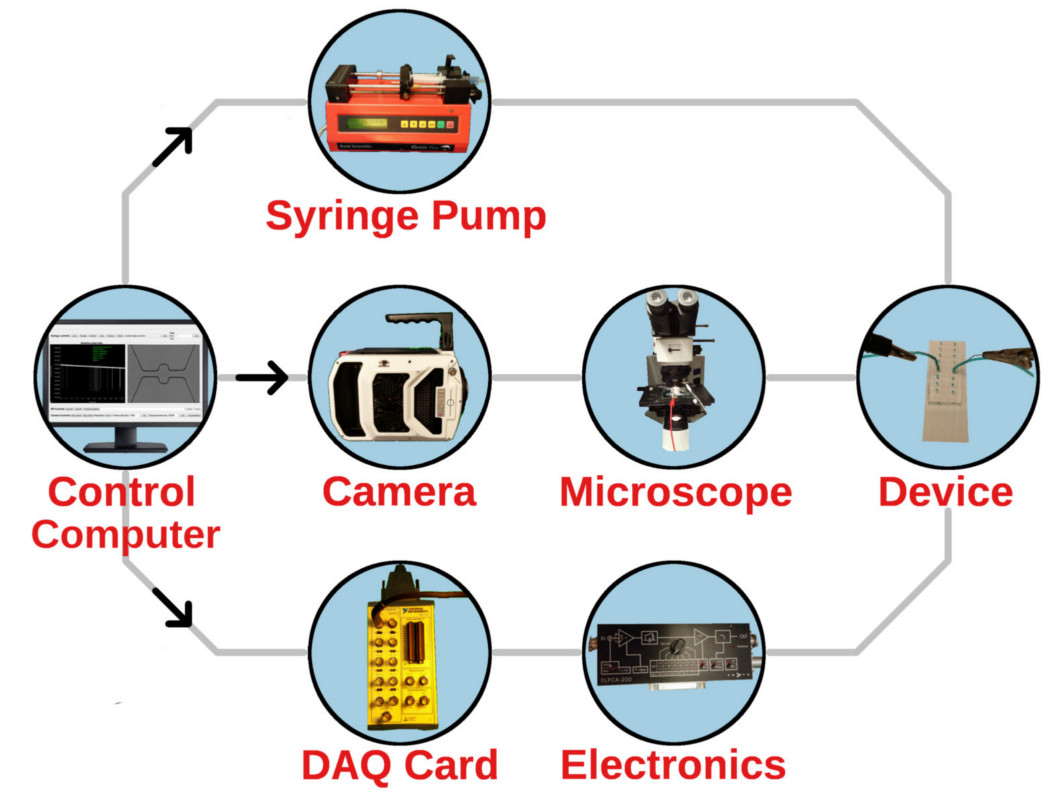
\includegraphics[width=\textwidth]{hardware.jpg}
			\caption{\textbf{Hardware set up for the hybrid RP-IM experiments.}}
			\label{fig:hardware}
		\end{figure}

	
		We devised a hybrid resistive pulse-optical imaging platform that is capable of resolving the spatial dependencies of the RP amplitude signals. The set up (Fig. \ref{fig:hardware}) consists of a high-speed camera combined with an optical microscope, all of the electronic equipment used to acquire the RP signal, a syringe pump to drive particle suspensions through the system, a planar microfluidic channel, and a central control computer used to run the experiment and record data.
		
		\begin{figure}
			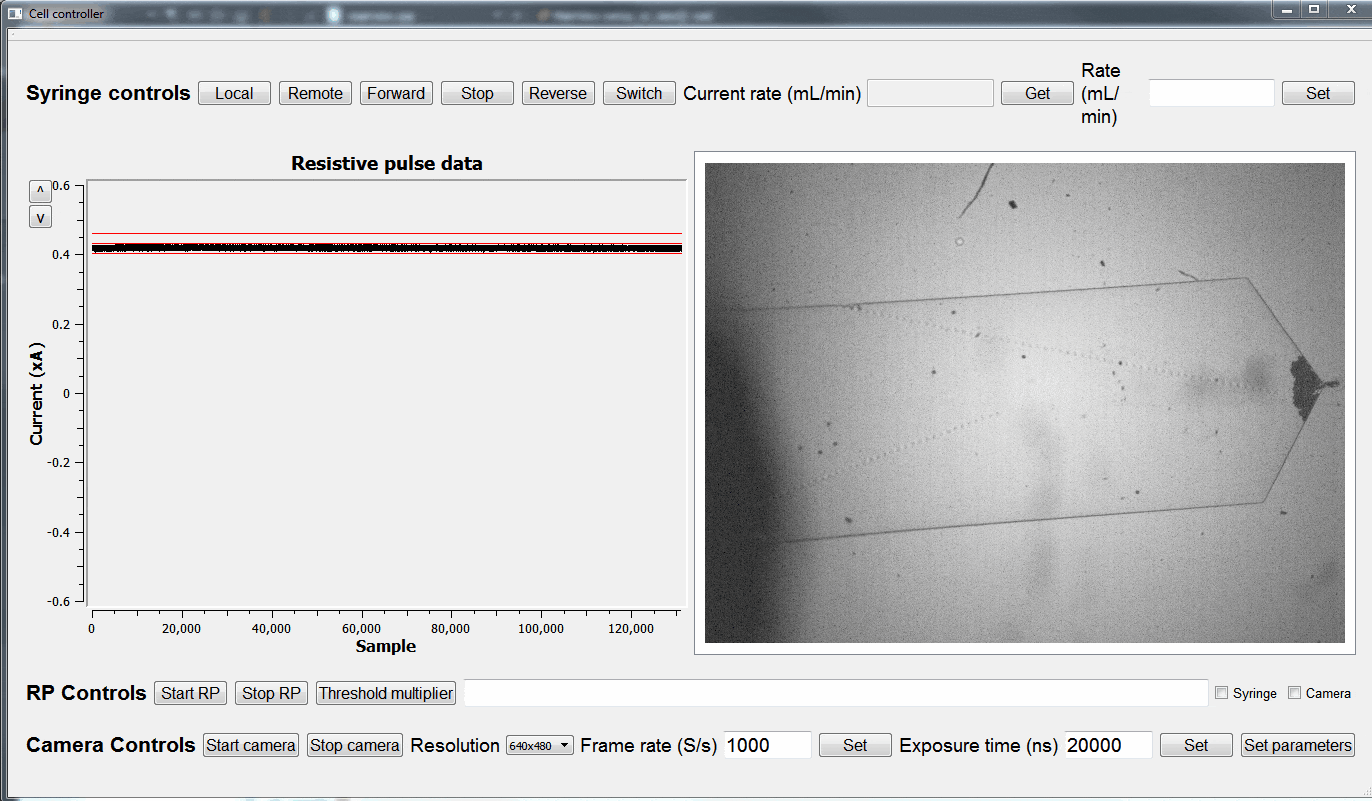
\includegraphics[width=0.5\textwidth]{cellcontroller.png}
			\caption{\textbf{\textit{cell\_controller}, a GUI program written in C++ and the Qt Framework}. The program controls the instruments used to run the experiment.}
			\label{fig:cellcontroller}
		\end{figure}

		
		The program used to control each of the instruments used in the experiment was written in C++ and makes use of the Qt framework to provide a GUI environment in which to run the experiment. The program is open-sourced and available at https://github.com/tphinkle/cell\_controller. The software controls the high-speed camera, a data acquisition (DAQ) card used to record the current measurements, and the syringe pump. Each instrument uses its own communication protocol; the high-speed camera is controlled by commands sent via TCP/IP protocol over a 1 GB/s ethernet line, the DAQ card is controlled using the National Instruments NIDAQmx API, and lastly, the syringe pump is controlled via serial commands sent over an RS-232 line. A screen shot of the program is shown in Fig. \ref{fig:cellcontroller}.
		
		The channels used for these experiments were made from PDMS bonded to a glass slide. PDMS is a transparent elastomer that is relatively inert, transparent, and durable, and for these reasons is probably the most common material used in microfluidic experiments today. Two classes of channels were created in PDMS, constant-width and variable-width, which will be discussed separately in the discussion section. Within each class of channels, different geometries were considered. Images of some of the channels used in the experiments are shown in Fig. \ref{fig:trajectories}, along with lines indicating the tracked trajectories of individual particles (discussed below). $\SI{10}{\mu m}$ polystyrene beads were used as the experimental particle to track, and were suspended in $\SI{1}{M}$ unbuffered KCl solution. The high concentration of solution was chosen because it increases the signal-to-noise ratio, and facilitates analysis of the RP events. The syringe pump rate was chosen to be $\SI{0.005}{mL/min}$, which enabled a large number of events to be detected while also allowing for good sampling of individual events in both the RP ($\SI{250,000}{kHz}$) and IM ($\SI{50,000}{kHz}$ sample, $\SI{10}{\mu s}$ exposure) signals. At this flow rate, particles traveled a small ($\SI{<10}{\mu m}$) distance in between frames, and minimal blurring occured. The \textit{cell\_controller} program recorded the camera and resistive pulse data simultaneously so that the two data streams are guaranteed to capture the same particle translocations.
		
	\section{Data analysis software}
		
		\begin{figure}
			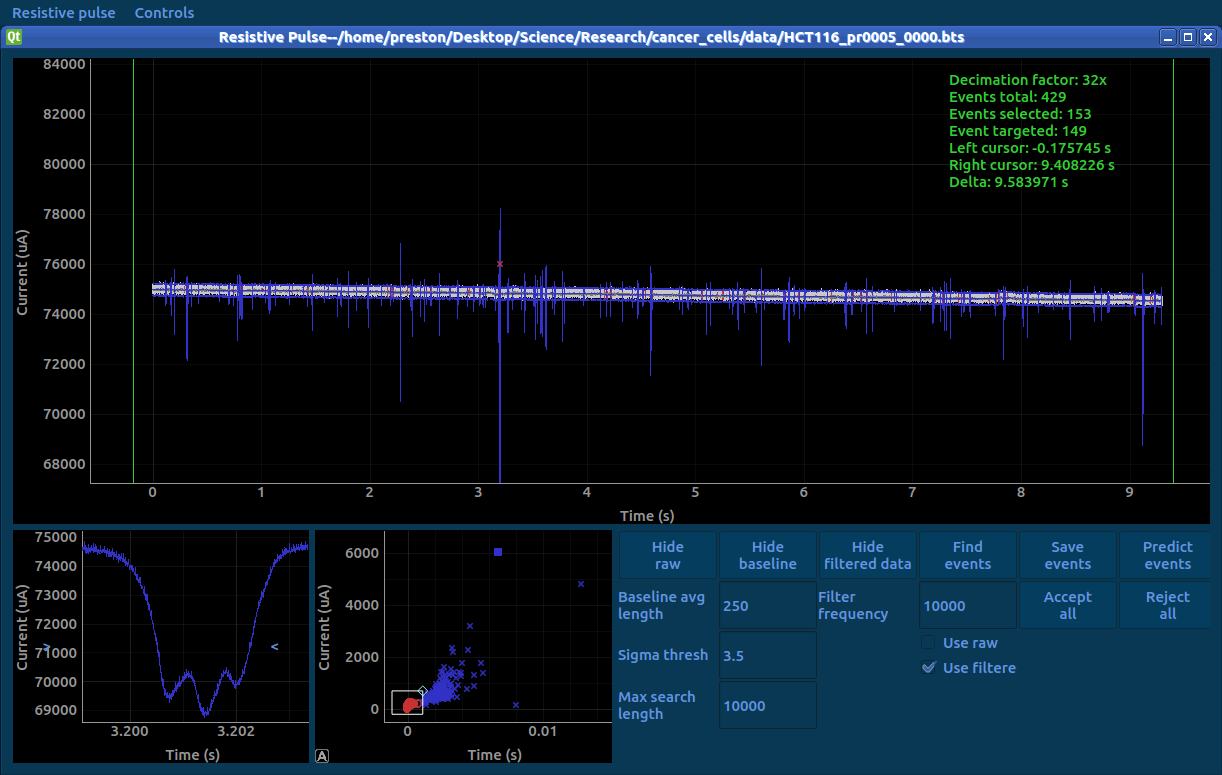
\includegraphics[width=\textwidth]{porestats}
			\caption{\textit{Screen capture of the GUI component of the \textit{pore\_stats} software library.} The program enables fast and accurate extraction of RP events from the baseline data. The main panel shows the raw time-series data (zoomed out), with events that were detected with the program highlighted in blue. The bottom left plot shows a single event that has been targeted by the user. The bottom right plot shows a scatterplot of the current and duration for all events detected, and shows how bulk events can be rejected by selecting a region of the scatter plot. The bottom right buttons and fields are used to change the search parameters, to begin the search, filter data, and enable various other functionalities.}
			\label{fig:porestats}
		\end{figure}

		
		A software library called \textit{pore\_stats} was written in Python and PyQt to facilitate analysis of the resistive pulse data. The program includes a GUI application that can be used to quickly isolate the resistive pulses from the entire time-series. The application includes a number of convenient aspects, including the ability to find events in a drifting or unsteady baseline, the ability to low-pass filter the data to find events with a low signal-to-noise ratio, the ability to filter events based on their amplitude and duration, and a function that allows the user to train a logistic regression model in order to make automatic future accept/reject predictions. A screenshot of the program is shown in Fig. \ref{fig:porestats}. Aside from the GUI program, \textit{pore\_stats} contains a wide variety of functions contained in a library that can be called to perform operations on the RP data, such as filtering, minimum/maximum detection, etc., and to calculate the relevant RP parameters such as duration, amplitude, sub-amplitudes, number of events, event velocity, etc. Finally, because the experiments used for this project include simultaneous resistive pulse and optical tracking, the \textit{pore\_stats} library contains modules for analyzing the imaging data. The library enables detection of particles in individual frames, tracking of particles across frames, and a host of image processing tools that allow the user to calculate physical parameters of interest, such as particle size, aspect ratio, position, etc.
		
	\section{Results \& Discussion}
		
		\subsection{Data analysis explanation}
		
		The experimental hardware and software, and the data analysis software described above were used to perform the experiments and analyze them completely. The data analysis pipeline is as follows. First, the resistive pulse data was opened using the GUI application within the \textit{pore\_stats} library, which was used to extract the detected RP events. Once RP events were detected in the baseline of the time-series, they were saved separately. Next, the camera images were analyzed in order to track optical events. Particles were detected within individual frames using a thresholding approach; a frame in which no particles were present was used as a template, which was subtracted off individual frames. This subtraction yields an image where the pixels of the particles are highlighted white, and everything else is black. A flood-fill algorithm was then used to find incidences of connected pixels, which correspond to individual particle detections. Then, this analysis was performed on hte next image in the camera's recorded video, and particles detected in this frame are connected with particles in the previous frame using a minimum-distance approach. Because we know the exact geometry of the channel, we are also able to determine the physical length of a pixel in the camera image. This is useful because we can then measure distance in physical units (e.g. microns) instead of pixel units. Additionally, we can also use the lines of the channel to create a coordinate system with axes aligned with the axial and lateral directions of the channel. The end result is that through the coordinate transformation and particle tracking, we are able to calculate the actual trajectory in physical units that a particle undertakes when passing through a channel. The trajectory is then described by a sequence of pairs $x_{c}, y_{c}$, where $x_{c}$ are the axial and $y_{c}$ transverse coordinates of the particle with respect to the channel's coordinate frame, in physical units of microns. We chose a coordinate system such that $x_{c}=0$ corresponds to the particle crossing the channel's threshold, and $y_{c}=0$ on the channel's axis.
		
		
		Because the particles travel very small distasnces in between frames, tracking individual particles across multiple frames is relatively straight forward. A string of individual detections comprises an IM event. In order to compare the events tracked via RP and IM, a protocol had to be established for matching the events appropriately. In order to do this, we first constructed two time series corresponding to the times of events of the tracked RP and IM signals. The times from one signal ewre shifted until both sequences were seen to overlap. In many cases tracking of some particles fails in either signal. For instance, in the RP signal there could be a brief burst of noise that prevents detection of a pulse in the baseline. In the camera data, failure to track a single particle was less likely to occur, although still possible in principle. Unpaired events were dropped from the respective sequence to which they belonged. After this coarse alignment, we are left with two sequences $IM$ and $RP$ such that every event $i$ in one signal has a matching event $i$ in the other signal that is known to correspond to the same physical particle translocation. However, in order to compare actual data points in the RP and IM signals, a more fine-tuned alignment must be made. In order to perform this exact matching, we find two data points that are known to correspond to the same instant in time (up to the precision of the slower of hte two instruments' sampling periods). For instance, for a pair of detected events in the RP and IM signals, we find the camera frame where the particle occupies the exact center of the channel, and the middle-most data point in the RP signal; we know that both data points correspond to the same instant in time (again, with precision given by the slower of the two sampling periods). Fine alignment of the two time series for each event is then achieved by adding a ismple time offset to one of the signals, equal to the difference in times of the two corresponding data points. In principle, if the camera and DAQ card sampled at exactly the rates specified by their hardware specifications, and this rate did not change within a single recording, fine alignment of the entire time-series would be possible by simply aligning the RP and IM data of a single particle translocation. However, in practice we find that if we apply this offset for a single particle, the signals become out of sync at a later time, which is due to slight inaccuracies in their reported sampling periods. For this reason, we do not apply a single shift to hte time-series in order to align the entire thing, but apply a unique alignment for every pair of events that we compare.
		
		\begin{figure}
			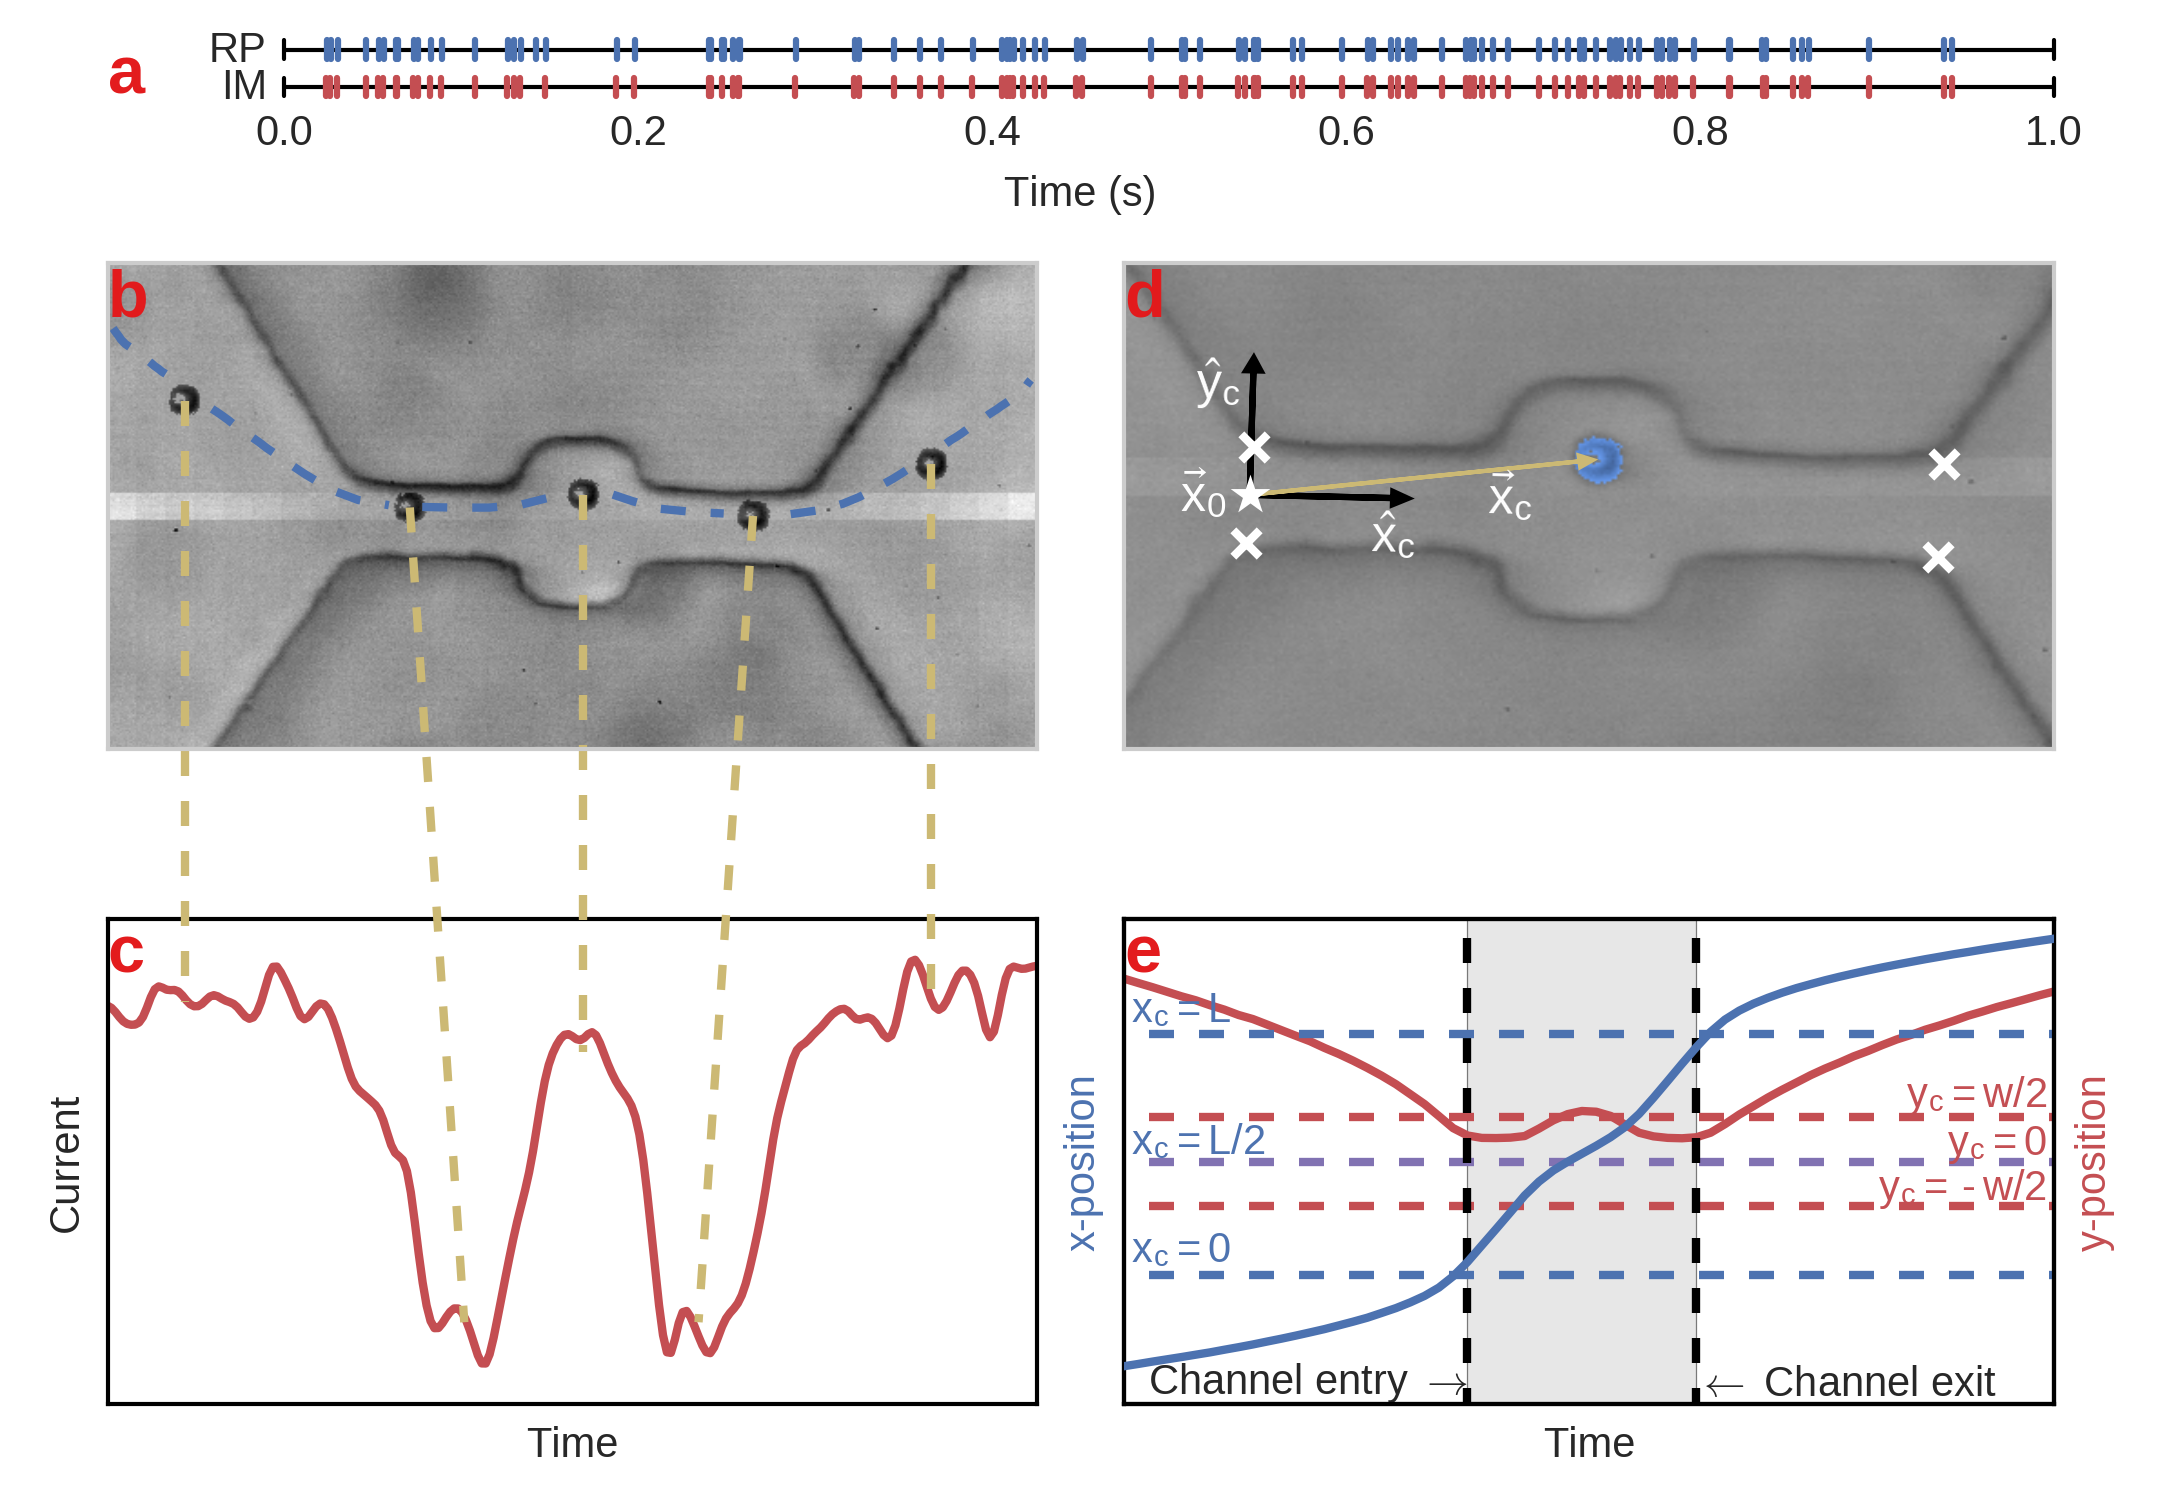
\includegraphics[width=1\textwidth]{rpimsync}
			\caption{\textbf{Event matching protocol for the RP and IM signals}. \textbf{a}.}
			\label{fig:rpimsync}
		\end{figure}

		
		After aligning the two time-series and calculating the position of the particle in the channel's coordinate system, we have a time-series of data $x, y, \Delta I/I_{p}$; in other words, for every event we are able to determine the exact $\Delta I/I_{p}$ for every position in the particle's trajectory through the channel. The event matching protocol, as well as calculation of the particle's positions in the channel's coordinate frame, are shown in Fig. \ref{fig:rpimsync}



%%% Local Variables: ***
%%% mode: latex ***
%%% TeX-master: "thesis.tex" ***
%%% End: ***
